\section{Event selection}
\label{sec:event_selection}
    %% Trigger selection
Events for this analysis are collected using a single HLT path, which is seeded by either a 20 \GeV or a 22 \GeV single \Pe/\Pgg\xspace L1 trigger depending on the running period. The HLT is used to select events with at least one photon with \et$ > 30$\GeV within the ECAL barrel region ($|\eta^{\gamma}| < $ 1.44) and calorimetric \met $ > $25 \GeV with noise cleaning to supress the anomalous noise in the HCAL barrel (HB) and endcap (HE) subdetectors due to characteristics of the hybrid photodiodes and the readout boxes~\cite{hcalnoise}. The trigger further requires the photon to pass a loose calorimeter-based isolation selection and to exhibit shower shape characteristics consistent with unconverted photons. The main shower shape requirement is based on the $R_{9}$ variable, defined as the ratio of the energy deposited in a $3\times 3$ crystal region centered around the crystal containing an energy deposit greater than all of its immediate neighbours (the ``seed crystal'')  to the energy of the entire deposit of the photon (``supercluster''). The data recorded with this trigger corresponds to an integrated luminosity of 7.3\fbinv and was part of the CMS ``data parking'' program in 2012. With the data parking program, CMS recorded additional data with relaxed trigger requirements planning for a delayed offline reconstruction in 2013 after the completion of the LHC Run I. %With the data parking program, CMS recorded and stored additional data with relaxed trigger requirements. The raw data was reconstructed after the completion of the first LHC run in 2013.

 The efficiencies of the trigger as a function of offline reconstructed \etg and \met are measured using two prescaled control trigger paths. The first control trigger path accept events with single photons with energy greater than 30 \GeV with no further identification or isolation requirements on the photons. The second control trigger path has identical photon requirements to the signal path but without any selection on \met. Figure~\ref{fig:triggereff} shows the efficiency turn-on curves as a function of \etg and \met, parameterized with an analytic function in the form of:

\begin{equation}                                                                                                                                                                  
\label{eq:acc}                                                                                                                                                                    
        \varepsilon = \frac{p_2}{2} \cdot \left( 1 + \text{Erf}\left(\frac{x - p_0}{p_1 \cdot \sqrt{2}}\right)\right).
\end{equation}            

%% figure for trigger efficiency and parameterization
\begin{figure}[!h]
\centering
{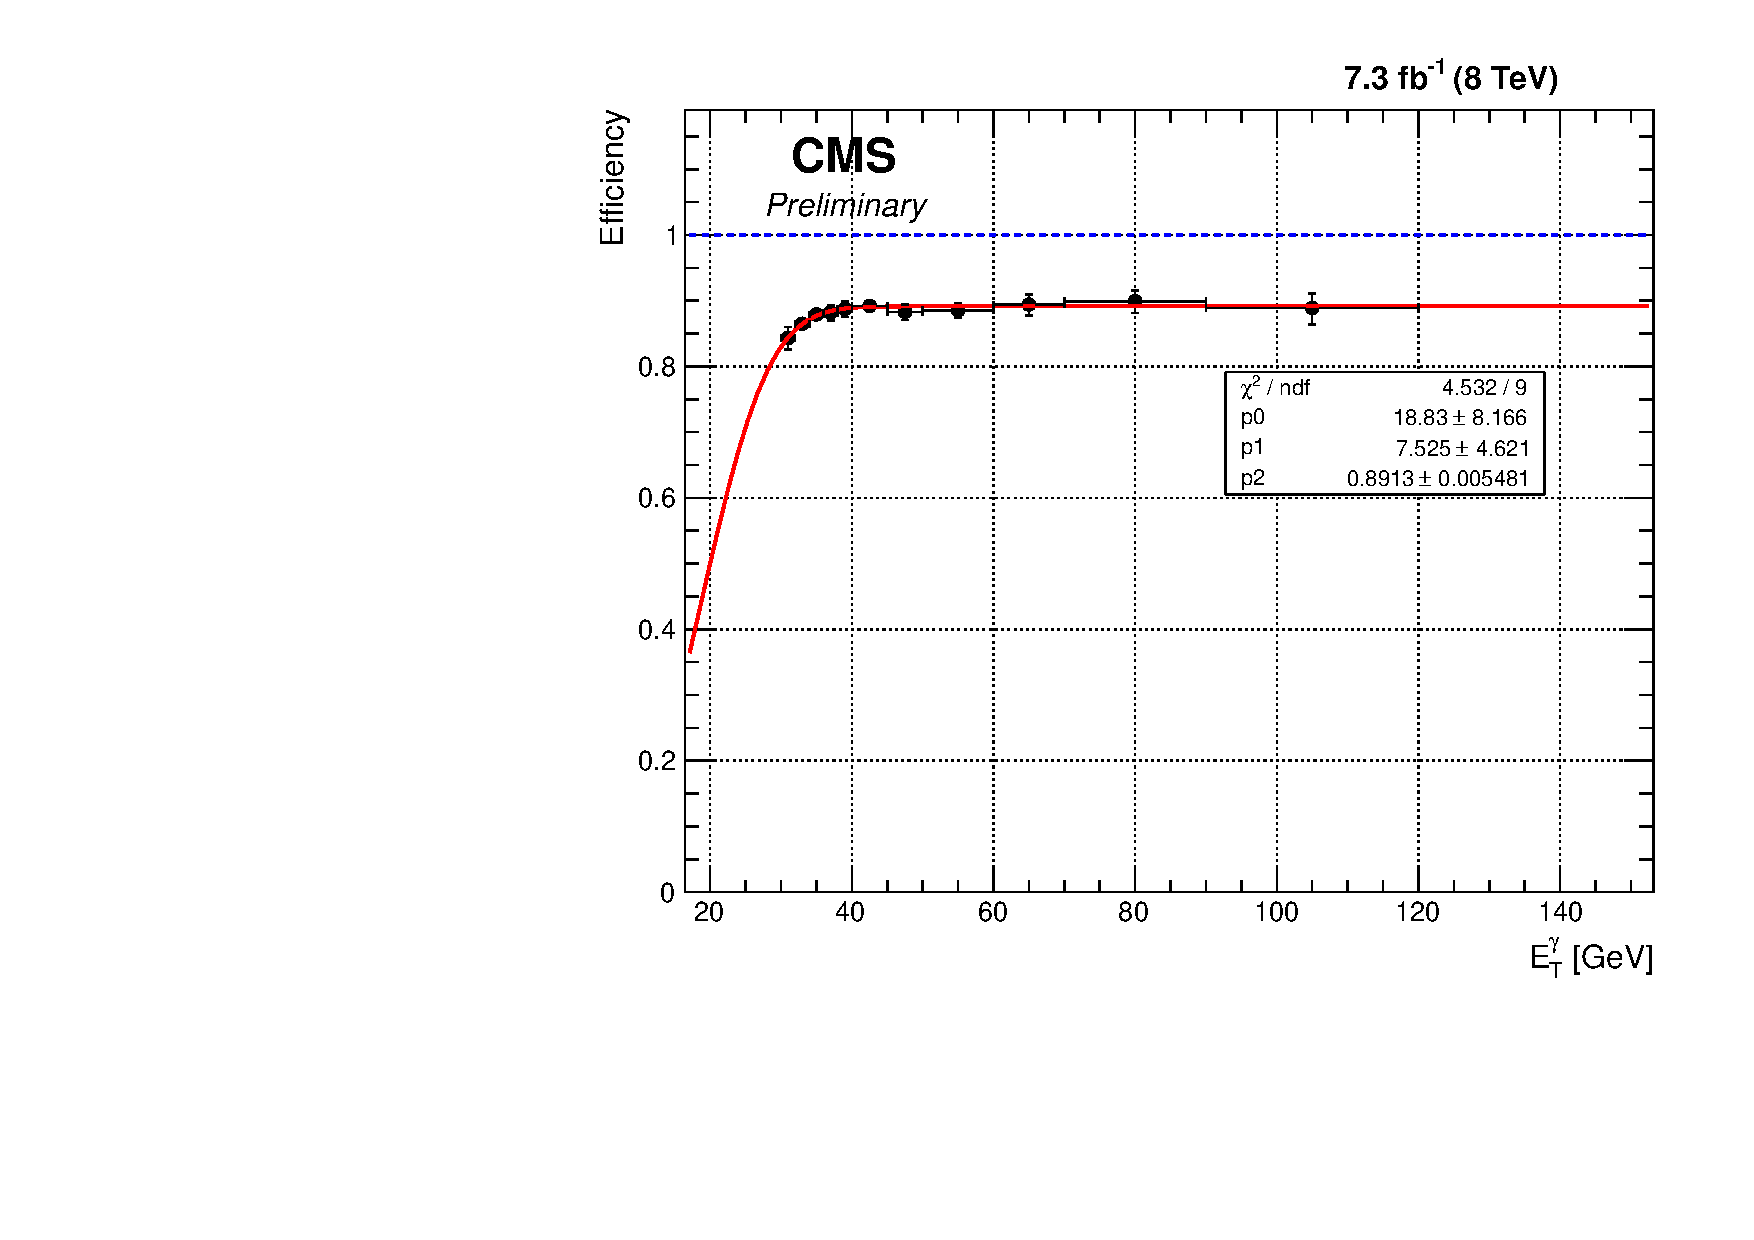
\includegraphics[scale=0.35]{figures/range_updated_photon.pdf}}
{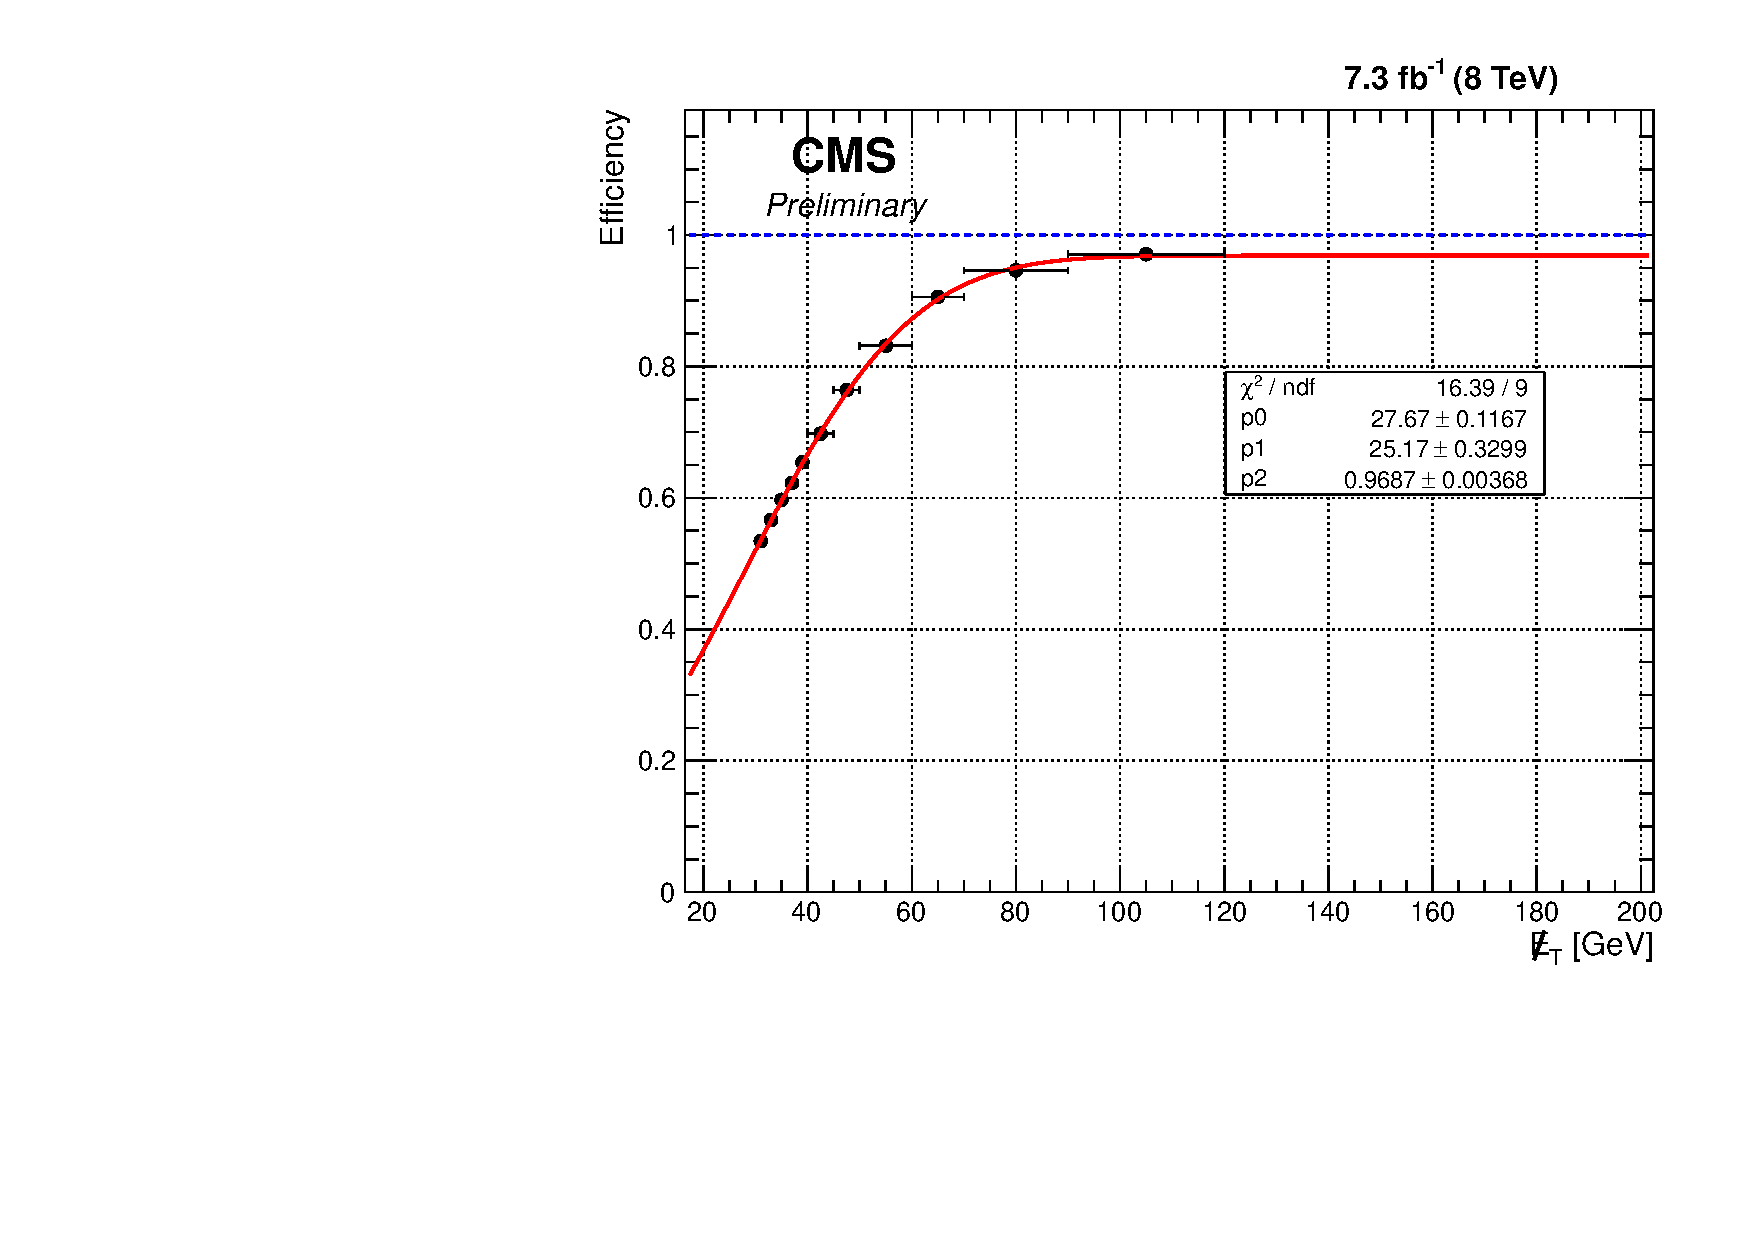
\includegraphics[scale=0.35]{figures/range_updated_met.pdf}}
%[]{\label{fig:triggPt}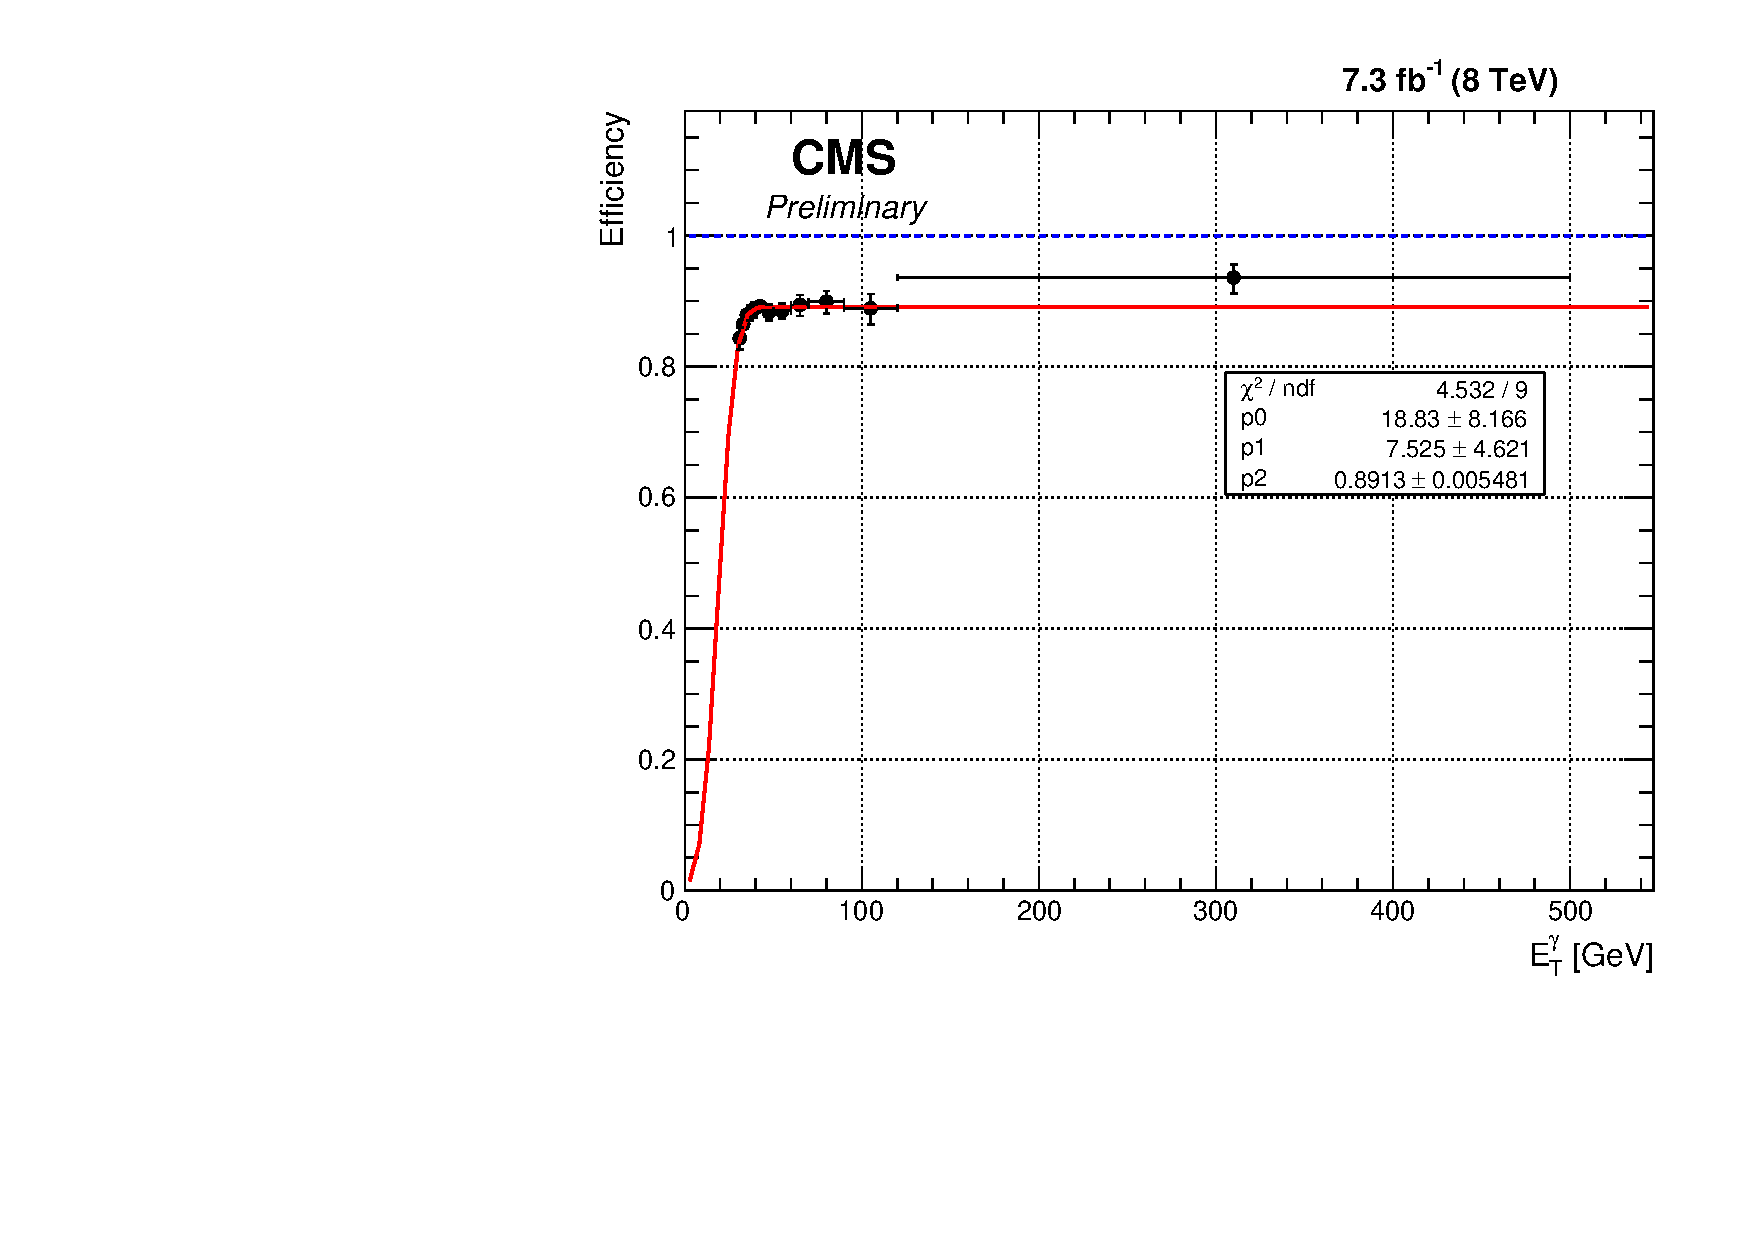
\includegraphics[scale=0.35]{figures/updated_photon.pdf}}
%[]{\label{fig:triggMET}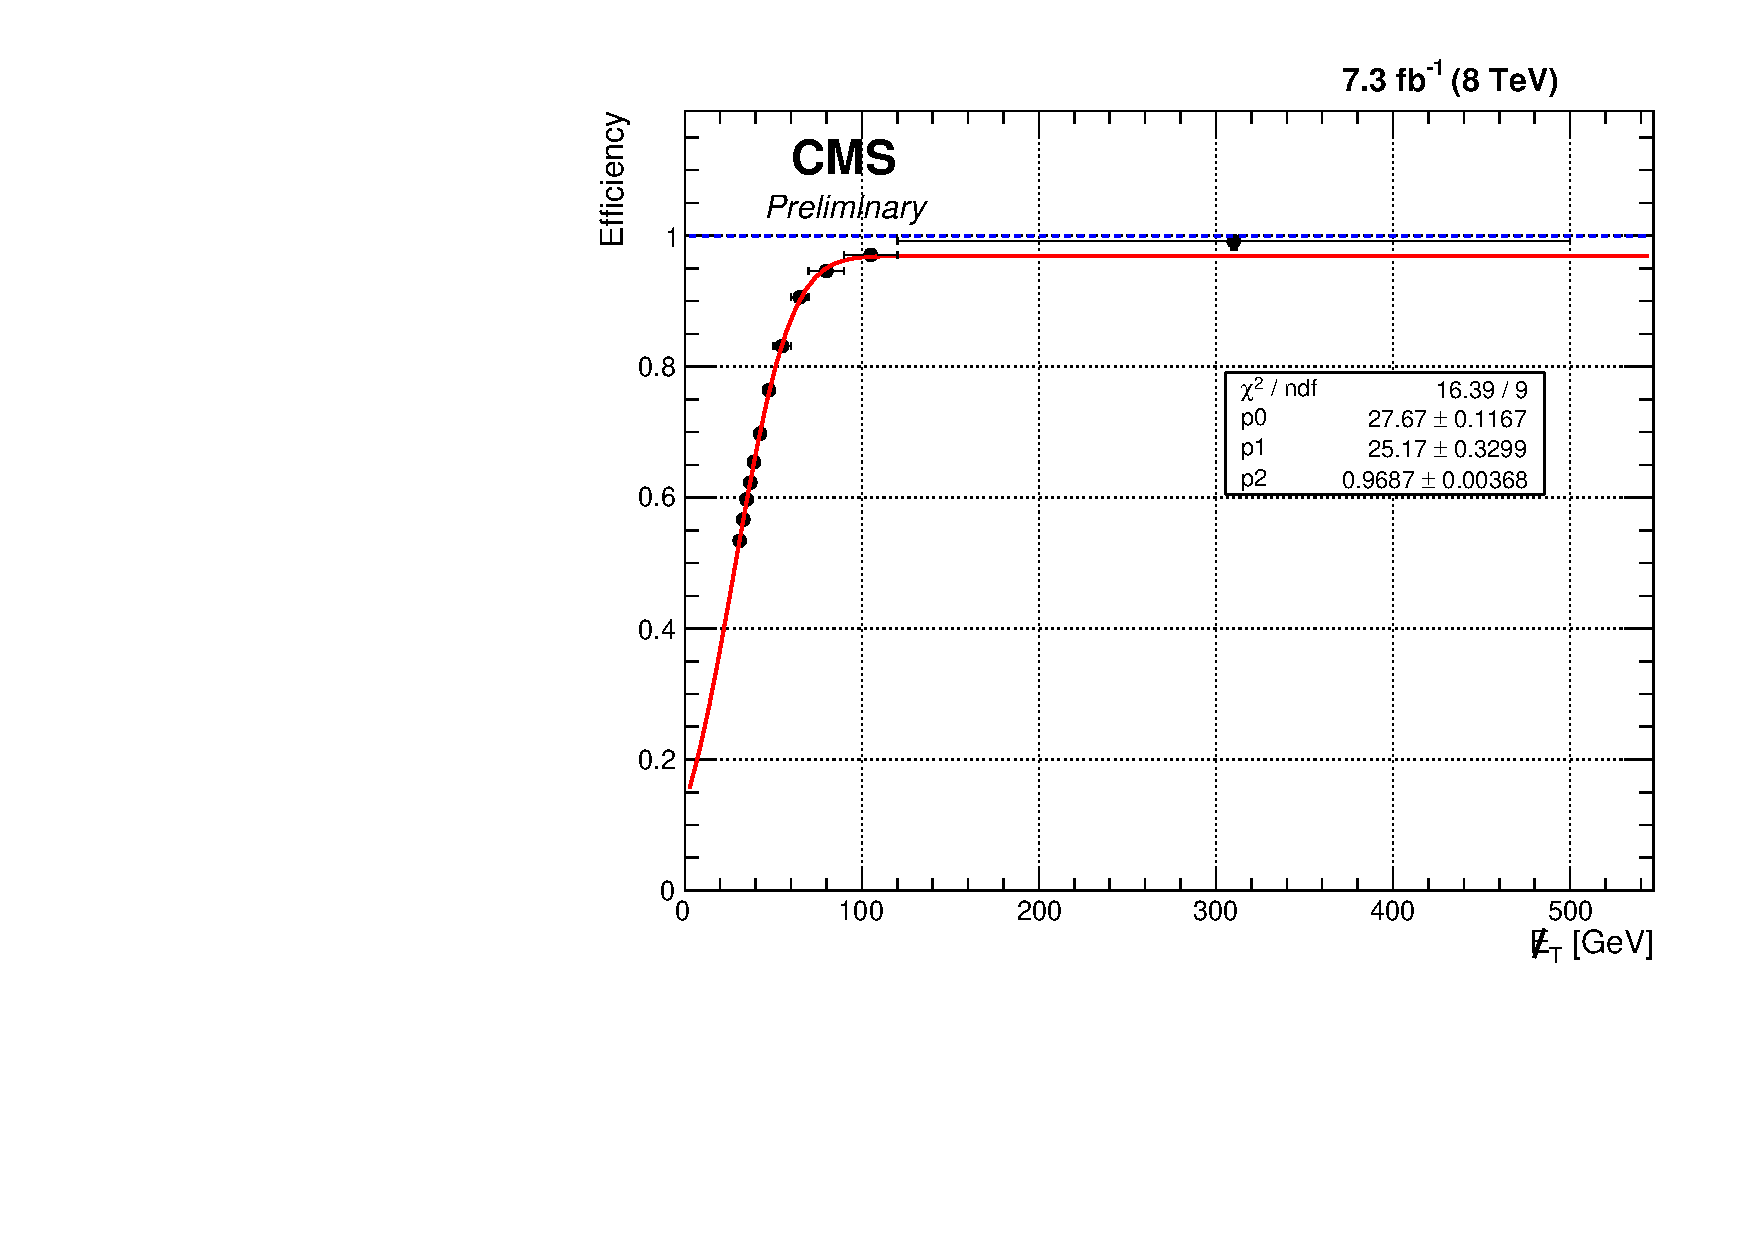
\includegraphics[scale=0.35]{figures/updated_met.pdf}}
\caption{Trigger turn-on curves for \etg and \met. The parameterization of efficiency as a function of offline \etg and \met are also shown in the form of an analytic function fitted to the turn-on distributions.}
\label{fig:triggereff}
\end{figure}
    %% Cleaning of Event

    In the offline selection, the events are required to have at least one well identified vertex with a distance less than 24 \cm away from the nominal interaction point in $z$-direction and 2 \cm away in the $xy$-plane. The vertex corresponding to the origin of the hard-scattering process with the largest value of $\sum \pt^2$ of all associated tracks is identified as the primary vertex.

    %% Photon selection
    Each selected event is required to have at least one photon candidate with  \etg\ $ > 45 \GeV$ and $|\eta^{\gamma}| < 1.44$.
		The photon must also satisfy the following identification and isolation criteria:
		(a) to minimize the contribution from misidentified electrons, the shower is required to have no associated hits in the pixel detector, to be referred to as "pixel seed veto";
		(b) the lateral extension of the shower, $\sigma_{i\eta i\eta}$, measured in terms of the energy-weighted spread within the $5\times 5$ crystal should be consistent with that of a genuine photon;
		(c) the ratio between the energy collected by the HCAL cells behind the supercluster and the energy collected by the supercluster is required to be less than 0.05;
		(d) the sum of the \et of all photons reconstructed with the particle flow (PF) algorithm within a cone of $\Delta R = 0.3$, excluding a strip in $\eta$ of 0.015 around the supercluster, is required to be less than $0.7 \GeV +0.005 \times$ \etg;
		(e) the sum of the \et of all charged hadrons reconstructed with the PF algorithm within a hollow cone of $0.02 < \Delta R < 0.3$ around the supercluster is required to be less than $1.5 \GeV$;
		(f) the sum of the \et of all neutral hadrons reconstructed with the PF algorithm within a cone of $\Delta R = 0.3$ around the supercluster is required to be less than $1.0 \GeV +0.04 \times$ \etg.
		To account for the effects of overlapping proton-proton interactions (pileup), the total energy density in the event is computed using the {\sc FastJet} package~\cite{Cacciari:2011ma} and is used to correct the isolation quantities.
		These pileup corrected isolation requirements correspond to a working point with a signal efficiency of approximately $85\%$. Furthermore, $R_{9} > 0.9$ is also required to match the trigger requirements.
		The photon with the highest \et in the event that satisfies all of the above requirements is selected as the photon candidate for the signal sample.

		Anomalous signals in the ECAL, due to direct interaction of particles with the ECAL photodiodes, are rejected using additional shower shape requirements on the $\eta$ and $\phi$ width of the shower. In addition, we reject showers that deposit more than 95\% of their energy on the seed crystal~\cite{spikecleaning}.  
% ($\sigma_{i\eta i\eta} > 0.001$)
%($\sigma_{i\phi i\phi} >  0.001$) 

    %% Veto of Electron and Jet
        To reduce the SM backgrounds arising from the leptonic decays of W and Z bosons, a lepton veto is applied. Events are rejected if they have at least one electron fulfilling a loose identification requirement~\cite{ele_id} with $\pt^{e} > 10\GeV$ and $|\eta^{e}| < 2.5$ (excluding the transition region of $1.44 < |\eta^{e}| \leq 1.55$) and are outside the cone defined by $\Delta R = 0.3$ around the photon candidate. Muons candidates which are identified using the PF algorithm using hits in the tracker and the muon systems are required to have $\pt^{\mu} > 10\GeV$, $|\eta^{\mu}| < 2.1$, and $\Delta R(\gamma,\mu) > $0.3 separation from the photon candidate. Events are rejected if any such muon is present in the event.

        In addition to the selection requirements described above, the \met is required to be greater than 40~\GeV. This level of selection is referred to as the preselection and is applied for both the model independent analysis and the analysis of the SUSY benchmark model. The additional applied selection requirements differ between the two analyses.
  
        To define the jet candidates, identification criteria are used to separate pileup jets from the jets originating from hard scattering. These identification criteria are based on the trajectory of tracks associated with the jets inside the tracker volume, the topology of the jet shape and multiplicity of the objects constituting these jets~\cite{CMS-PAS-JME-13-005}. Only jets with $\pt^{jet} > $30 \GeV and $|\eta^{jet}| < 2.4$ and that fulfill the non-pileup identification requirements are considered in the event. These jets must not overlap with photon candidate within $\Delta R(\gamma,$jet$) < 0.5$. In the model independent analysis, events with 2 or more jets are rejected and, if there is a jet in the event, we also require that $\Delta \phi(\gamma,$jet$) < 2.5$. 

% new MHT
	    In the analysis of the SUSY benchmark model, where no requirement is made on the jet multiplicity, more advanced selection is applied to reduce the background due to mismeasured \met. Mismeasured \met can arise from many sources, including limited \met resolution, reconstruction and instrumental inefficiencies, and improper pattern recognition. Due to their large cross section the $\gamma + $ jets and multijet processes can contribute significantly to the background of this analysis, even though such events do not have genuine \met. In order to minimize the contribution from these processes, we have used two different methods for identifying events with mismeasured \met. The first one is  the \met significance method ~\cite{Chatrchyan:2011tn} which takes into account the reconstructed objects in each event and their known measurement resolutions to compute an event-by-event estimation of the likelihood that the observed \met is consistent with zero. To complement this method we further developed the Missing $\HT$ (M$\HT$) minimization method~\cite{CMS:2014mea}. In the M$\HT$ minimization method we first construct a $\chi^2$ function with the form:
 
\begin{equation}\label{eq:1ab}
   \chi^2 = \sum_{i=objects} \left( \frac{(\PT^{reco})_i-(\widetilde{p}_{\mathrm{T}})_i}{(\sigma_{\PT})_i} \right)^2 + \left( \frac{\widetilde{\Em}_x}{\sigma_{{\Em}_x}}\right)^2  + \left( \frac{\widetilde{\Em}_y}{\sigma_{{\Em}_y}}\right)^2.
\end{equation} 
In the above equation, $(\PT^{reco})_{i}$ are the transverse  momenta of the reconstructed objects that pass the above mentioned identification criteria, the $(\sigma_{\PT})_{i}$ are the expected resolutions of each object, the $\sigma_{{\Em}_{x,y}}$ are the resolution of the \met projection along the x-axis and the y-axis and the $(\widetilde{p}_{\mathrm T})_{i}$ are the free parameters allowed to vary in order to minimize the function. The first term of the equation is a scalar difference. The quantities $\widetilde{\Em}_{x,y}$ are functions of the free parameters;
  
\begin{eqnarray}
\widetilde{\Em}_{x,y} =  - \sum_{i=objects} (\widetilde{p}_{x,y})_i %\nonumber
 %&=&  \Em^{reco}_{x,y} + \sum_{i=objects} (p_{x,y}^{reco})_i-(\widetilde{p}_{x,y})_i \\
\end{eqnarray}

    In events with no genuine \met, the mismeasured quantities can be re-distributed back into the particle momenta, resulting in a low $\chi^{2}$ value. On the other hand, in events with genuine \met from undetected particles, the minimization generally will yield larger $\chi^{2}$ values. For the analysis of the SUSY benchmark model, the re-calculated $\widetilde{\met} = \sqrt{\widetilde{\Em}_{x}^2 + \widetilde{\Em}_{y}^2}$, i.e., in which the original object momenta are replaced with those obtained with the $\chi^{2}$ minimization, is required to be $ > 45$ GeV and the probability value obtained from the $\chi^{2}$ minimization is required to be less than $10^{-3}$. %It should be noted that the $\widetilde{\met}$ met can be reviewed as a correction on the $\met$ energy scale. 

    To further suppress multijet backgrounds, events are rejected if the scalar sum of transverse momentum of the identified jets (\HT) in the event is required to be greater than 100 \GeV. An additional requirement is made on the angle ($\alpha$) between the beam direction and the major axis of the supercluster in order to reject photons that have showers elongated along the beam line which is characteristic of non-prompt photons. 

    Finally, the transverse mass, $M_{T} = \sqrt{2 \pt^{\gamma} \met (1-\cos\Delta\phi(\gamma,\met))}$, formed by the photon candidate, \met and the angle between them,  is required to be greater than 100 \GeV. In order to easily interpret the results within the chosen benchmark model, we require the \etg$ < $60\GeV.
	%The selection \etg$ < $60\GeV, in addition to \etg$ > $45\GeV, effectively reduces the additional background that could arise from production of top squark exchange in low-scale SUSY-breaking models or resonant production of $Z\rightarrow \PXXSG\PSGczDo$~\cite{Petersson:2012dp,Achard:2003tx}.

	The final list of advanced selection used in both the model independent analysis and the analysis of the SUSY benchmark model with the relative cumulative efficiencies of the selection requirements relative to the preselection is given on table \ref{tab:cuts}. 
	
	 
\begin{table}[htbp]
\scriptsize
\setlength\extrarowheight{2pt}
\centering
%\begin{tabular}{|c|c|c|}
\begin{tabular}{|c|*{2}{c|}*{3}{c|} }
\hline
Selection requirements	&  \multicolumn{2}{|c|}{Model ndependent} & \multicolumn{3}{|c|}{SUSY benchmark model} \\\hline
\hline
%\emph{Preselection} & $Z\Pgg\rightarrow\Pgn\Pagn\Pgg$ & $\Pgg$+jet & $Z\Pgg\rightarrow\Pgn\Pagn\Pgg$ & $\Pgg$+jet & $M_{\PSGczDo} = 70 \GeV$ \\\hline
%\multicolumn{3}{|c|}{\emph{Preselection}}		\\\hline
%\hline
%Trigger Selection and Event Cleaning & XX & XX & X & XX & XX  \\\hline
%Photon Identification and Isolation		& XX & XX & X & XX & XX  \\\hline
%\etg\ $ > 45$ \GeV			& XX & XX & X & XX & XX  \\\hline
%$\met > 40$ \GeV				& XX & XX & X & XX & XX  \\\hline
%Lepton veto					&  & XX & X & XX & 99.94\%  \\\hline
%\hline
\emph{Advanced selection} & $Z\Pgg\rightarrow\Pgn\Pagn\Pgg$ & $\Pgg$+jet & $Z\Pgg\rightarrow\Pgn\Pagn\Pgg$ & $\Pgg$+jet & $M_{\PSGczDo} = 120 \GeV$ \\\hline
\hline
Number of jets $< 2$ & 0.909 & 0.769 & - & - & -  \\\hline
$\Delta \phi(\gamma,$jet$) < 2.5$			& 0.834 & 0.262 & - & - & -  \\\hline
Transverse mass $> 100$~\GeV	& - & - & 0.867  & 0.292 & 0.829  \\\hline
\HT $<  100$~\GeV				& - & - & 0.785 & 0.188 & 0.804  \\\hline
M$\HT$ minimization: $\widetilde{\Em}_T > 45$~\GeV 	& - & - & 0.761 & 0.071 & 0.743 \\\hline
M$\HT$ minimization: Prob($\chi^2$)$  < 10^{-3}$	& - & - & 0.626 & 0.033 & 0.467  \\\hline
$\met$ significance $>  20$			& - & - & 0.440 & 0.001 & 0.195  \\\hline
$\alpha >  1.2$					& - & - & 0.390 & 0.001 & 0.165  \\\hline
\etg\ $ < 60$~\GeV		& - & - & 0.074 & 0.0002 & 0.106  \\\hline
\end{tabular}
\caption{Summary of selection for both model independent analysis and analysis with SUSY benchmark model with the cumulative efficiencies of the selection requirements relative to the preselection for $Z\Pgg\rightarrow\Pgn\Pagn\Pgg$ , $\Pgg$+jet and $M_{\PSGczDo} = 120 \GeV$. }
\label{tab:cuts}
\end{table}
